\noindent

\includegraphics[height=1.25cm]{images/pictograms/replication}
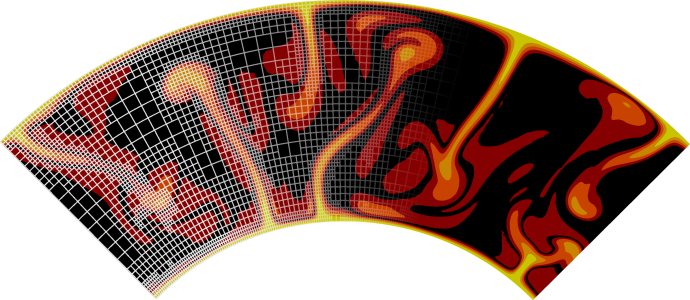
\includegraphics[height=1.25cm]{images/pictograms/aspect_logo}

\includegraphics[height=1.25cm]{images/pictograms/benchmark}

\includegraphics[height=1.25cm]{images/pictograms/pic}

%%%%%%%%%%%%%%%%%%%%%%%%%%%%%%%%%%%%%%%%%%%%%%%%%%%%%%%%%%%%%%%%%%%%%%%%%%%%%%%%%%%%%%%%%%%%%%%%%%%

\begin{flushright} {\tiny {\color{gray} python\_codes/fieldstone\_122/text.tex}} \end{flushright}

%\lstinputlisting[language=bash,basicstyle=\small]{python_codes/template_keywords.key}

\par\noindent\rule{\textwidth}{0.4pt}

\begin{center}
\inpython
{\small Code: \url{https://github.com/cedrict/fieldstone/tree/master/python_codes/fieldstone_122}}
\end{center}

\par\noindent\rule{\textwidth}{0.4pt}

%%%%%%%%%%%%%%%%%%%%%%%%%%%%%%%%%%%%%%%%%%%%%%%%%%%%%%%%%%%%%%%%%%%%%%%%%%%%%%%%%%%%%%%%%%%%%%%%%%%

This \stone is a replication of the benchmarks found in the supplementary material 
of \textcite{galh18} (2018): 

\begin{displayquote}
``We tested the accuracy of the implemented advection
schemes with two example models that separately show the
convergence of the integration error in spatially and temporally 
variable flow. Both models use an analytically prescribed 
velocity function that is evaluated and transferred
to the finite-element solution vector. By this procedure we
ensure that the particle algorithm behaves as in a normal
coupled computation, but retain full control over the velocity 
field that allows us to choose benchmarks with analytical
solutions, and are independent of the accuracy of the finite
element solver.''
\end{displayquote}

\begin{center}
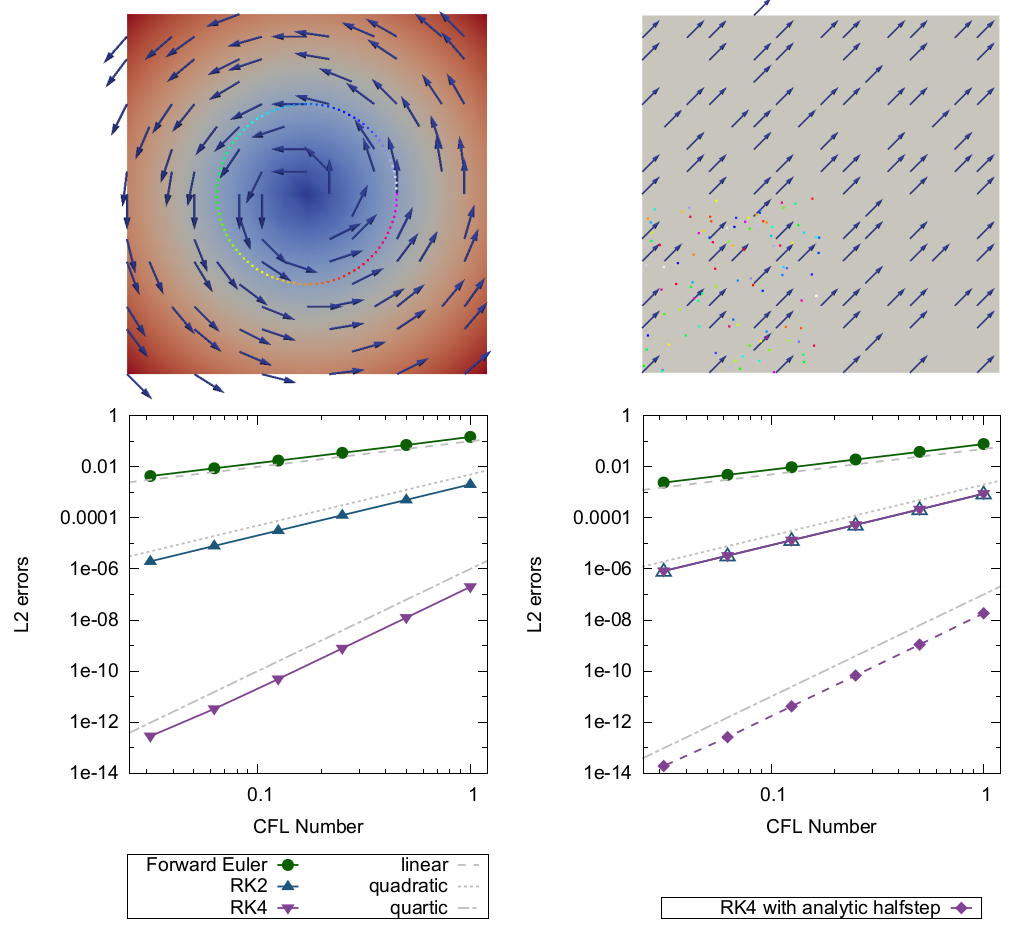
\includegraphics[width=11cm]{python_codes/fieldstone_122/images/galh18.png}\\
{\captionfont Taken from the supplementary material of \textcite{galh18} (2018). 
Left is benchmark \#1, with a rotational time-independent velocity field, Right is benchmark \#2
with a linear time-dependent velocity field.}
\end{center}

%%%%%%%%%%%%%%%%%%%%%%
\section*{Benchmark 1}

This benchmark is described as follows:
\begin{displayquote}
``The first benchmark model consists of a circular flow
around the center of a two-dimensional box. The model
end time and velocity of the flow is chosen to match one
turn-around time around the center. The model contains
100 particles that are distributed in a ring with a constant
radius around the model center. The error is measured as
distance between final and initial position that should approach 
zero in an analytical solution. To ensure that the
error is independent of the particle’s starting position we
plot the maximal error of all particles.''
\end{displayquote}

The code is quite simple. First a $nelx \times nely$ mesh of $Q_2$ elements
is created, alongside with its connectivity.
Then 100 particles are placed in an equidistant manner on a circle or radius 1, placed in
the middle of the $2\times 2$ domain. Then a velocity field $\vec\upnu=(y-2,-x+2)$ is used to 
advect these particles. 
Various Runge-Kutta methods are implemented, i.e. RK1, RK2, RK3, RK4, RK4(3/8), RKF and ODE87 
(see Section~\ref{MMM-ss:rkm}).

When a CFL number is chosen, the corressponding timestep is computed from the mesh size and velocity field.
Since the velocity on the circle has a magnitude of 1, then the total time needed to do a $2\pi$ 
circumference (radius is 1) is given by $t_f=2 \pi$. The number of time step is then $nstep=t_f/dt$, rounded 
to the nearest integer. Finally I recompute $dt=tfinal/nstep$ to make sure that particles 
come back exactly to their original position (exact $2\pi$ rotation)\footnote{In retrospect I should
have done like in the paper, i.e. adapting the velocity to achieve the desired CFL.}.

When the option {\python interpolate} is False, the velocity is computed on each particle and at 
any sub-timestep using the analytical velocity and here are the results\footnote{These results are 
obtained on a 16x16 mesh but that is not so relevant since it is not used anywhere, except than 
for computing $dt$. Also, I only consider 1 particle out of 100 for simplicity.}:

\begin{center}
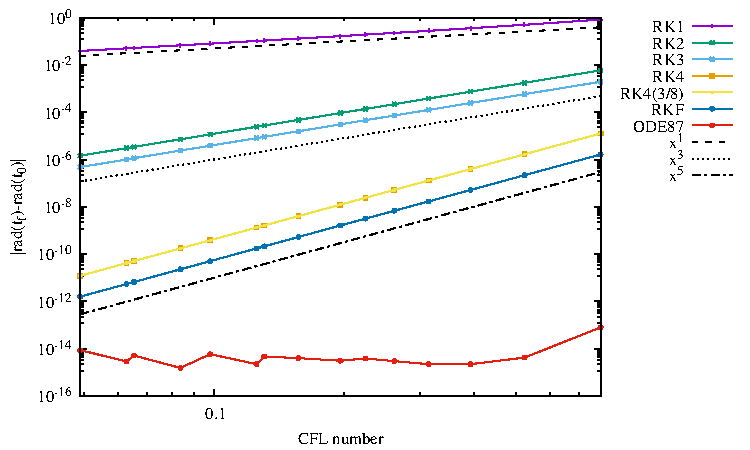
\includegraphics[width=5.7cm]{python_codes/fieldstone_122/results/exp1/errors.pdf}
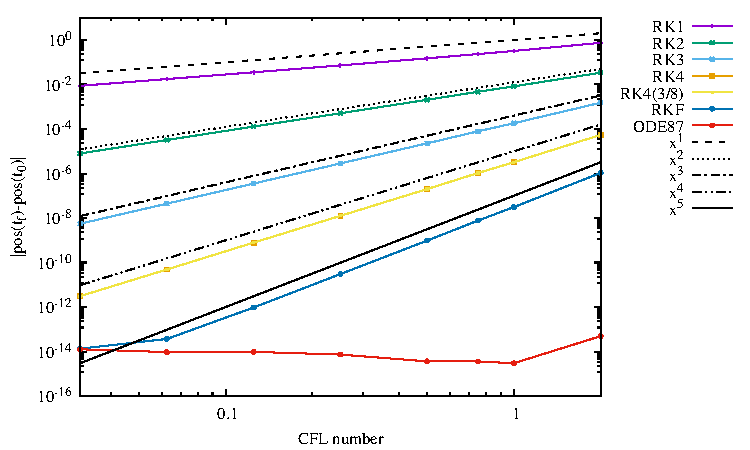
\includegraphics[width=5.7cm]{python_codes/fieldstone_122/results/exp1/errors2.pdf}
\includegraphics[width=5.7cm]{python_codes/fieldstone_122/results/exp1/rad.pdf}\\
{\captionfont Left: radius error as a function of the CFL number and for various RK methods for 
one particle; Middle: distance between starting point position and ending point position as a function of CFL number; 
Right: radius error as a function of time for a given CFL number of 0.5.}
\end{center}

I find that even order RK methods over perform for radius (distance to center of the circle) error, 
not sure I can explain this. When considering the distance between particles after $2\pi$ rotation, 
$r(t_f)-r(t_0)$, we recover the expected rates of \textcite{galh18}. 
Also, we find virtually no difference between RK4 and RK4(3/8) results.

The performance of ODE87 is remarkable (error at machine precision), but at a conservative 
CFL number of 0.5, RK4 is near $10^{-8}$. Given that a typical lengthscale for mantle modelling 
is $\sim 6000km$, then this is already an error of $\sim 10^{-5}km$, or $\sim 10^{-2}$m. 
In essence such a level of accuracy is not really needed in practice.

If I now first compute the velocity on the mesh and use the $Q_2$ basis functions to interpolate the 
velocity on the particles ({\python interpolate}=True), the code takes longer to run, as 
demonstrated by this code excerpt for RK1:
\begin{lstlisting}
for istep in range(0,nstep):
    for im in range(nmarker):
        if interpolate:
           ielx=int(swarm_x[im]/hx)
           iely=int(swarm_y[im]/hy)
           iel=iely*nelx+ielx
           rm=(swarm_x[im]-x[iconV[0,iel]])/hx-0.5
           sm=(swarm_y[im]-y[iconV[0,iel]])/hy-0.5
           swarm_r[im]=rm
           swarm_s[im]=sm
           swarm_iel[im]=iel
           NNNV=NNV(rm,sm)
           um=NNNV.dot(u[iconV[:,iel]])
           vm=NNNV.dot(v[iconV[:,iel]])
        else:
           um,vm=velocity(swarm_x[im],swarm_y[im])
        swarm_x[im]+=um*dt
        swarm_y[im]+=vm*dt
    # end for im
\end{lstlisting}

\newpage
Lookin at the results for various mesh resolutions, we get a totally different picture:

\begin{center}
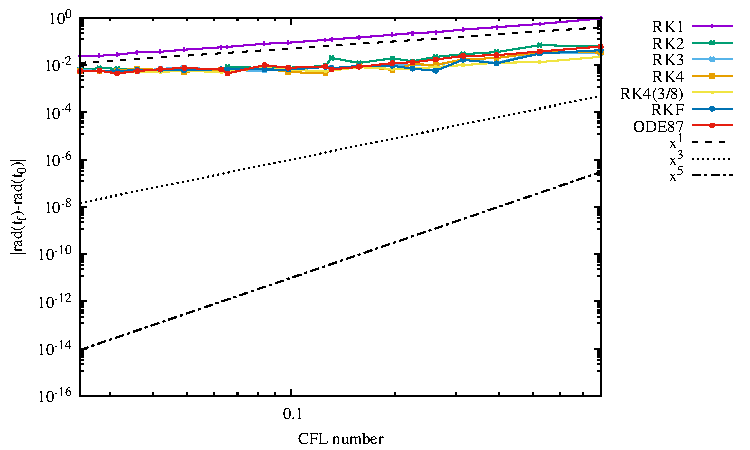
\includegraphics[width=5.7cm]{python_codes/fieldstone_122/results/exp1_16/errors.pdf}
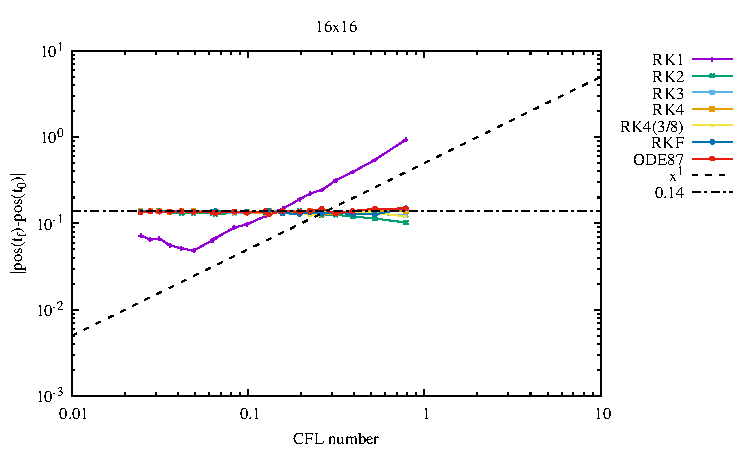
\includegraphics[width=5.7cm]{python_codes/fieldstone_122/results/exp1_16/errors2.pdf}
\includegraphics[width=5.7cm]{python_codes/fieldstone_122/results/exp1_16/rad.pdf}\\
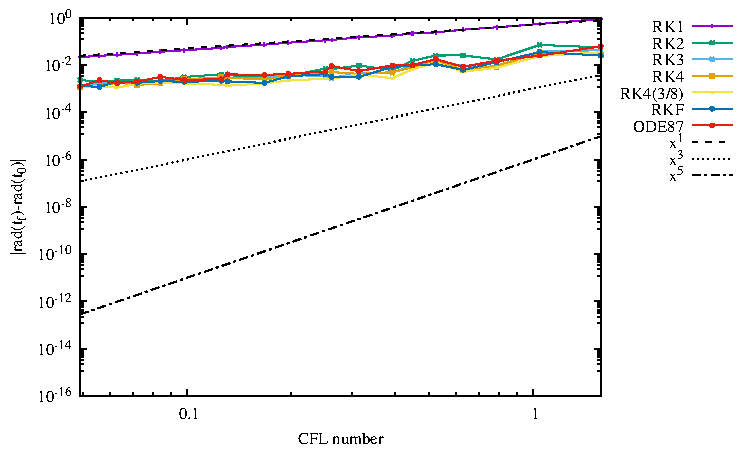
\includegraphics[width=5.7cm]{python_codes/fieldstone_122/results/exp1_32/errors.pdf}
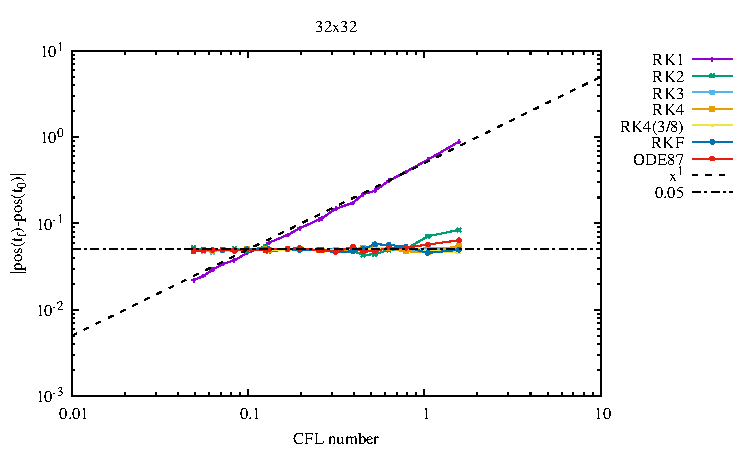
\includegraphics[width=5.7cm]{python_codes/fieldstone_122/results/exp1_32/errors2.pdf}
\includegraphics[width=5.7cm]{python_codes/fieldstone_122/results/exp1_32/rad.pdf}\\
\includegraphics[width=5.7cm]{python_codes/fieldstone_122/results/exp1_64/errors.pdf}
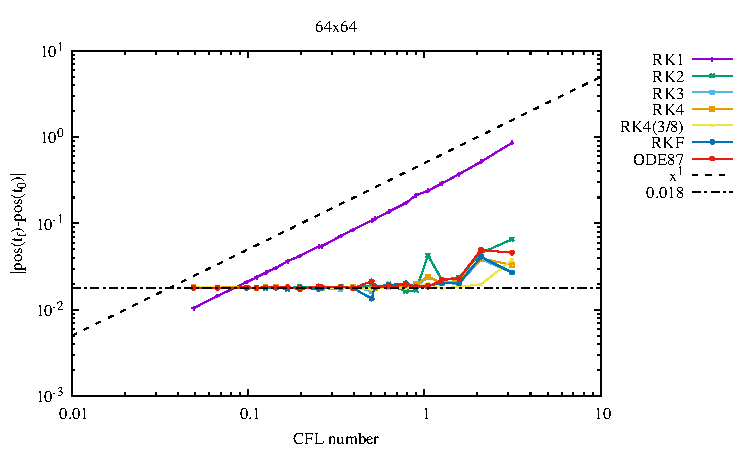
\includegraphics[width=5.7cm]{python_codes/fieldstone_122/results/exp1_64/errors2.pdf}
\includegraphics[width=5.7cm]{python_codes/fieldstone_122/results/exp1_64/rad.pdf}\\
\includegraphics[width=5.7cm]{python_codes/fieldstone_122/results/exp1_128/errors.pdf}
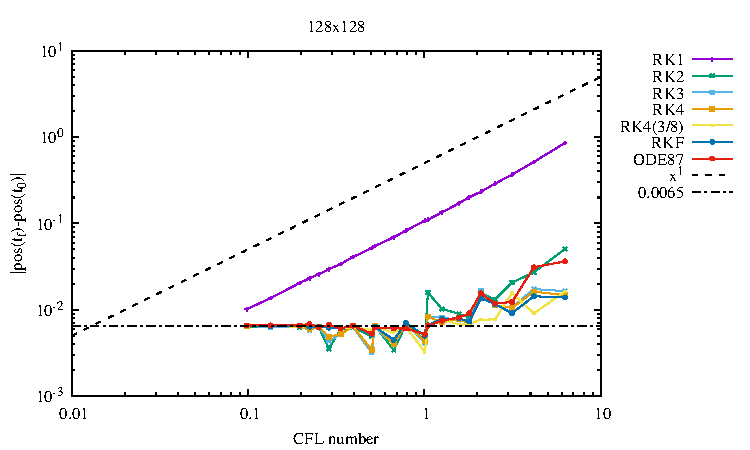
\includegraphics[width=5.7cm]{python_codes/fieldstone_122/results/exp1_128/errors2.pdf}
\includegraphics[width=5.7cm]{python_codes/fieldstone_122/results/exp1_128/rad.pdf}\\
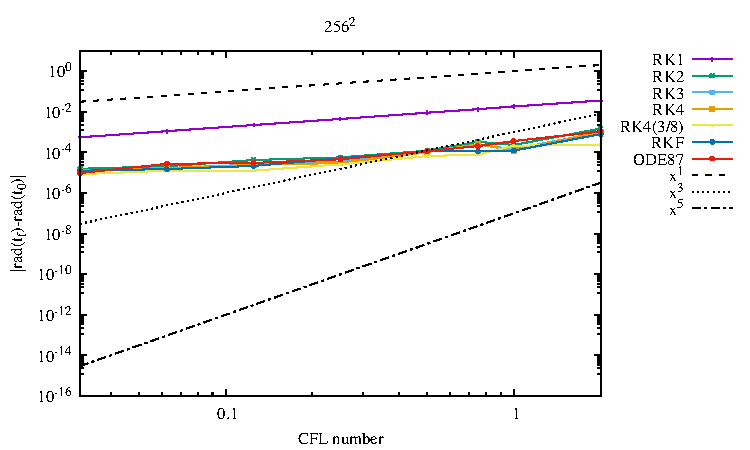
\includegraphics[width=5.7cm]{python_codes/fieldstone_122/results/exp1_256/errors.pdf}
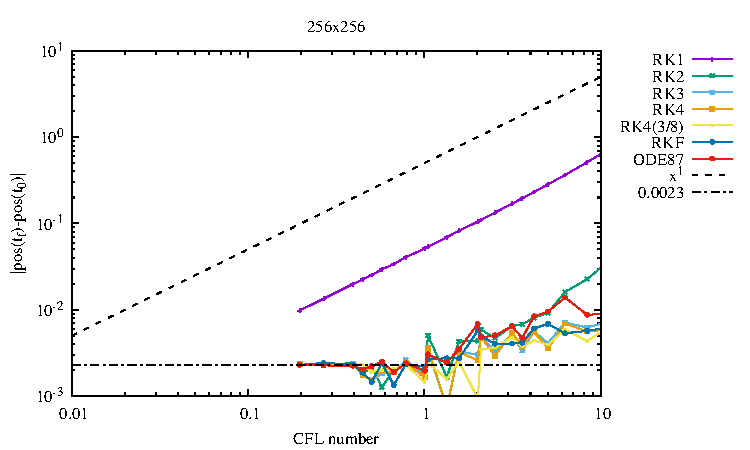
\includegraphics[width=5.7cm]{python_codes/fieldstone_122/results/exp1_256/errors2.pdf}
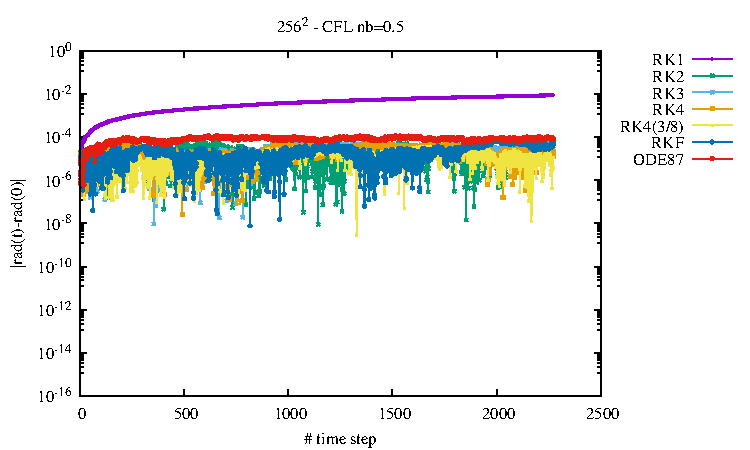
\includegraphics[width=5.7cm]{python_codes/fieldstone_122/results/exp1_256/rad.pdf}\\
{\captionfont From top to bottom: $nel=16^2,32^2,64^2,128^2,256^2$.}
\end{center}

We find that the error is then 100\% controlled by the mesh size, and high order methods do 
make any difference {\it all}.
The conclusion is that any method higher order than RK2 is probably pointless. 


\newpage
%%%%%%%%%%%%%%%%%%%%%%
\section*{Benchmark 2}

This benchmark is described as follows:
\begin{displayquote}
``The second benchmark model measures the convergence
in time-variable flow, which is simulated by a model domain 
with spatially constant but over time exponentially-
increasing velocity. All particles are generated at random
positions in the lower-left quadrant of the model domain
and are advected in a flow of the form
\[
u(t)=1 + e^t \qquad 
v(t)=1 + e^t 
\].
The model end time
of 1 then leads to an expected final
position $\vec{x}(1) = \vec{x}(0) + \int_0^1 \vec\upnu(t) \; dt$
 with a distance between the initial and end position of $d = ||\vec{x}_1-\vec{x}_0 ||_2 = 2e$.''
\end{displayquote}








